\documentclass[11pt, aspectratio=169]{beamer}
\usetheme{Madrid}
\usefonttheme{serif}

\usepackage[utf8]{inputenc}
\usepackage[T1]{fontenc}
\usepackage{subcaption}
\usepackage{cite}
\usepackage{amsmath}
\usepackage{amsfonts}
\usepackage{amssymb}
\usepackage{graphicx}

\usepackage[english]{babel}

\DeclareMathOperator{\sen}{sen}
\DeclareMathOperator{\tg}{tg}

\setbeamertemplate{caption}[numbered]
\usepackage[font=small,labelfont=bf]{caption}
\author[Group 3]{Group 3}
\title{Final: Hopfield Network}
% Informe o seu email de contato no comando a seguir
% Por exemplo, alcebiades.col@ufes.br
\newcommand{\email}{email}
%\setbeamercovered{transparent} 
\setbeamertemplate{navigation symbols}{} 
\logo{
\includegraphics[scale=0.06]{imagens/hcmus_logo.png}} 
\institute[]{VNUHCM - University of Science} 
\date{\today} 
%\subject{}

% ---------------------------------------------------------
% Selecione um estilo de referência
\bibliographystyle{apalike}

%\bibliographystyle{abbrv}
%\setbeamertemplate{bibliography item}{\insertbiblabel}
% ---------------------------------------------------------

% ---------------------------------------------------------
% Incluir os slides nos quais as referências foram citadas
%\usepackage[brazilian,hyperpageref]{backref}

%\renewcommand{\backrefpagesname}{Citado na(s) página(s):~}
%\renewcommand{\backref}{}
%\renewcommand*{\backrefalt}[4]{
%	\ifcase #1 %
%		Nenhuma citação no texto.%
%	\or
%		Citado na página #2.%
%	\else
%		Citado #1 vezes nas páginas #2.%
%	\fi}%
% ---------------------------------------------------------

\begin{document}

\begin{frame}
\titlepage
\end{frame}

\section*{Members}
\begin{frame}{Members}
    \begin{center}
      \begin{tabular}{@{}l@{}}
          \tabitem 23122001 - Dinh Duc Anh Khoa\\
          \tabitem 23122006 - Luu Thuong Hong\\
          \tabitem 23122008 - Mai Duc Minh Huy\\
          \tabitem 23122020 - Nguyen Thien An
        \end{tabular}
    \end{center}
\end{frame}



\begin{frame}{Table of contents}
\tableofcontents 
\end{frame}


\section{Introduction \& Why Hopfield Network?}
\subsection{Introduction}
\begin{frame}
\frametitle{1.1. Introduction}
\textbf{Associative Memory}
\begin{itemize}
    \item Retrieves patterns from partial or noisy input data, a foundational concept in machine learning.
\end{itemize}

\textbf{Core Characteristics}
\begin{itemize}
    \item A type of attractor network.
    \item Facilitates auto-association (pattern completion) and optimization tasks in neural networks.
    \item Operates as a Recurrent Neural Network (RNN) leveraging the Hebbian learning rule \cite{hertz1991introduction}.
\end{itemize}

\textbf{Limitations of Traditional RNNs}
\begin{itemize}
    \item Face performance bottlenecks and storage inefficiencies, addressed by the Hopfield Network.
\end{itemize}
\end{frame}

\subsection{Why Hopfield Network?}
\begin{frame}{1.2. Why Hopfield Network?}
\begin{itemize}
    \item Recognized by the Nobel Prize in Physics 2024.
    \item Integrates self-attention mechanisms in Transformers \cite{vaswani2017attention} \cite{ramsauer2020hopfield}.
\end{itemize}
\begin{figure}[H]
    \centering
    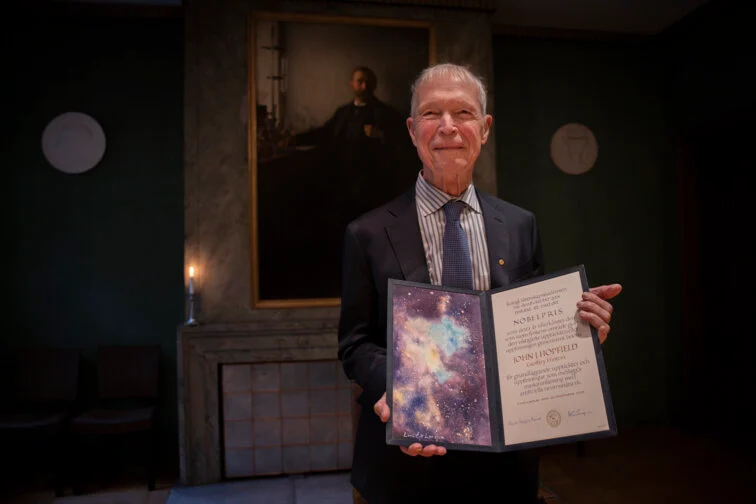
\includegraphics[width=0.5\linewidth]{imagens/hopfield_nobel.png}
    \caption*{\small{Photo: Nanaka Adachi}}
\end{figure}
\end{frame}

\section{Hopfield Network and the concepts behind it}
\begin{frame}{2. Hopfield Network and the concepts behind it}
    \begin{figure}
        \centering
        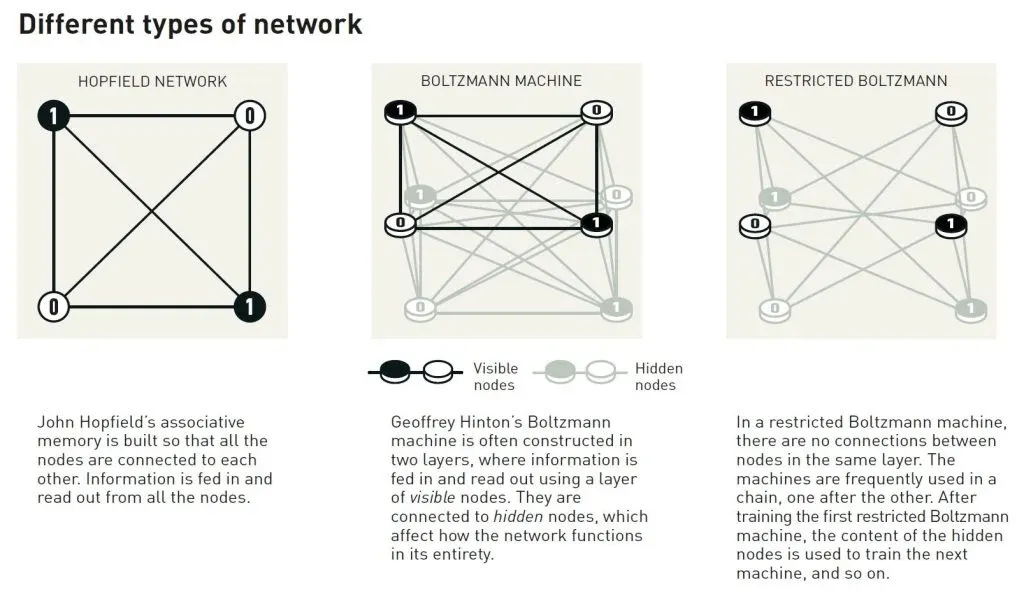
\includegraphics[width=0.75\linewidth]{imagens/types_network.png}
        \caption{Different type of network \cite{mediumBrainsPixels}}
        \label{fig:types_network}
    \end{figure}
\end{frame}
\begin{frame}{2. Hopfield Network and the concepts behind it}
The inspiration for Hopfield network comes from spin-glass systems in physics \cite{Müller1995}. Hebbian Learning shapes the energy landscape by creating deep wells at stored pattern locations. The network then transitions between states, with noisy inputs naturally rolling down to the nearest stored pattern.
\begin{figure}[H]
    \centering
    \begin{minipage}{.4\textwidth}
        \centering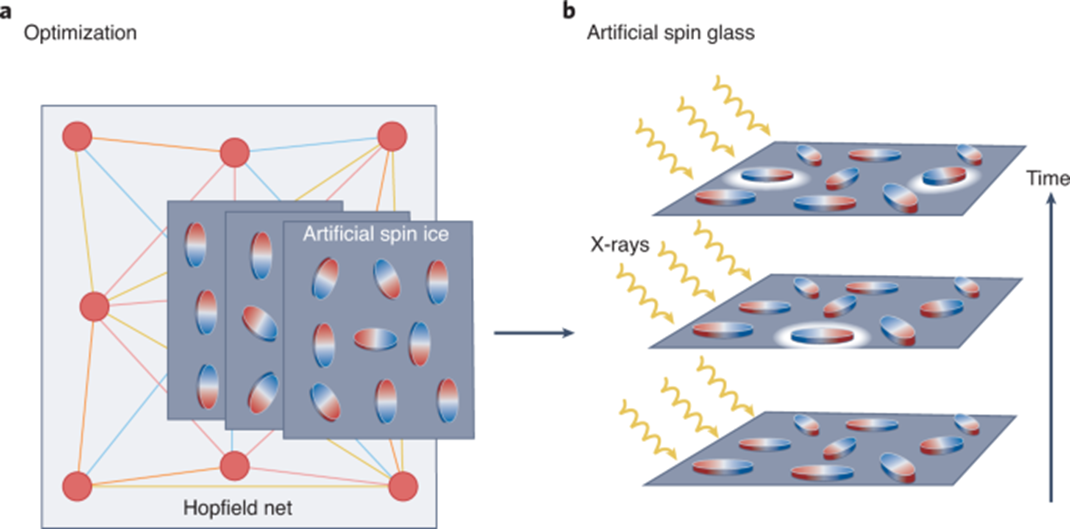
\includegraphics[width=1\linewidth]{imagens/glass_spin.png}
        \centering\caption*{Spin-glass system \cite{Makarov2022}}
        \label{fig:spinglass}
    \end{minipage}%
    \begin{minipage}{.6\textwidth}
        \centering
        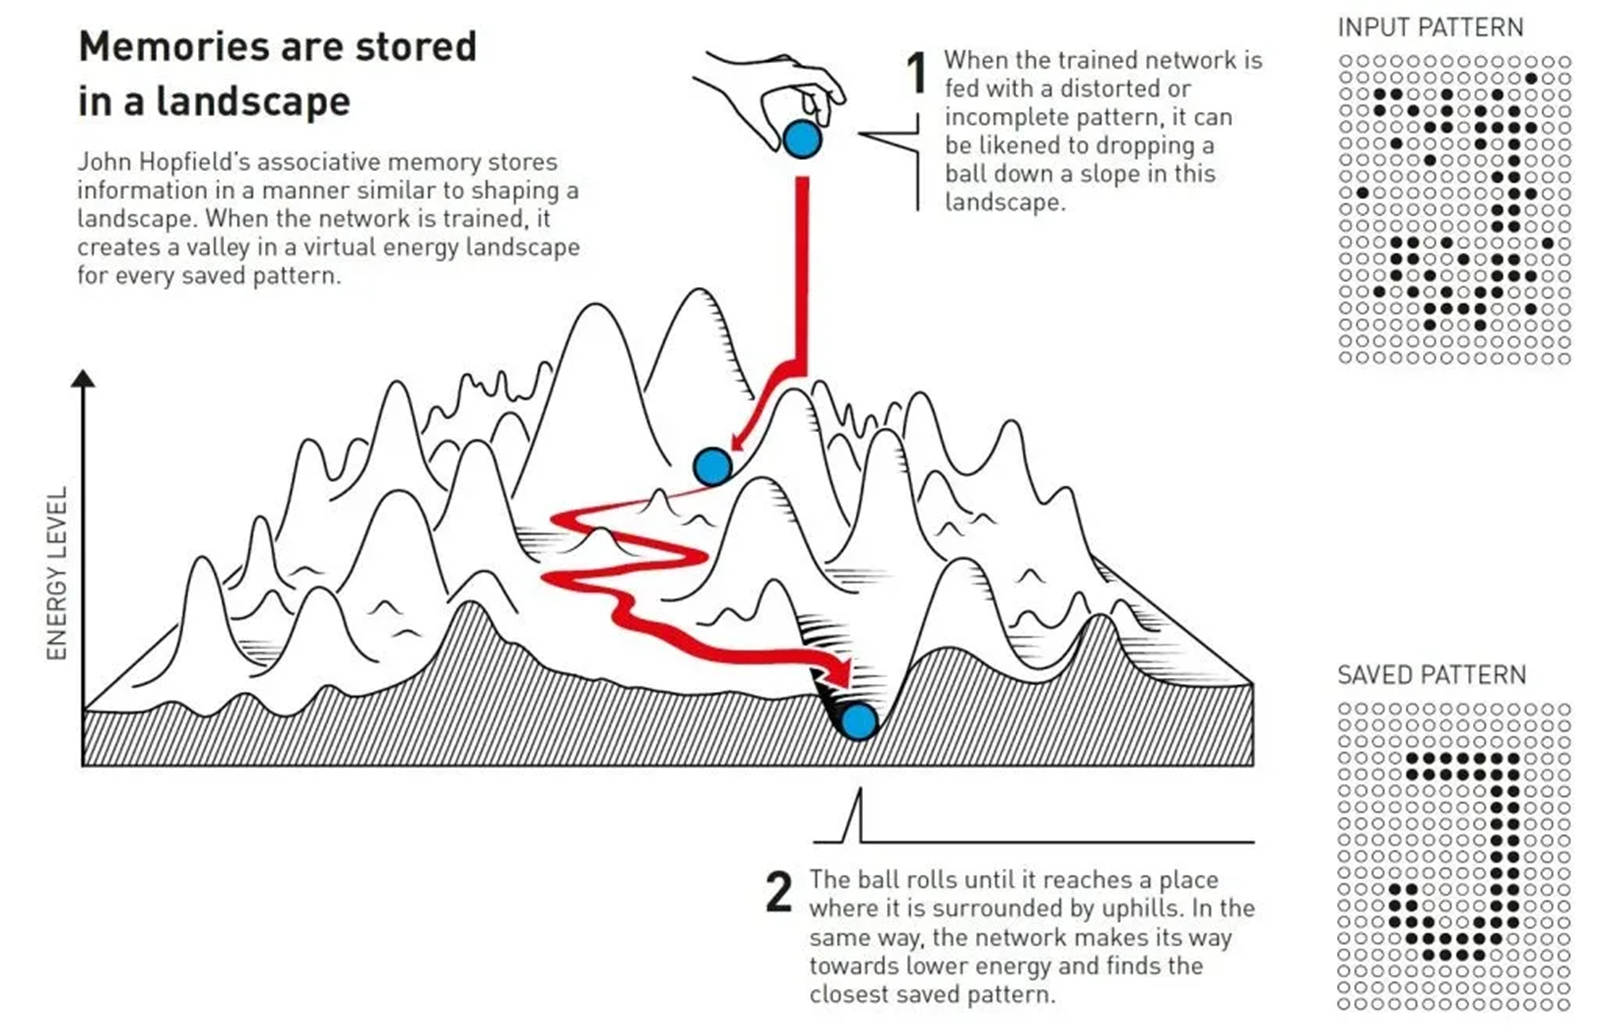
\includegraphics[width=0.8\linewidth]{Ball_rolling.png}
        \caption*{Energy Landscape \cite{mediumBrainsPixels}}
        \label{fig:landscape}
    \end{minipage}
\end{figure}
\end{frame}


\subsection{Free Energy Principle (FEP)}
\begin{frame}{2.1 FEP \cite{10.7551/mitpress/12441.001.0001}}
\begin{itemize}
\item Free energy is the difference between a system's predictions of upcoming inputs and the incoming inputs. \textit{(Equivalent to loss function)}
\item The free-energy principle states that biological systems (a neuron, the brain, …) will try to minimize free energy by \textbf{updating its model of the world toward better predictions} (KL-Divergence) OR \textbf{acting to change the world to agree with its model} (Action-based Inference).
\end{itemize}

\end{frame}

\begin{frame}{2.1 FEP \cite{10.7551/mitpress/12441.001.0001}}
\begin{figure}[H]
    \centering
    \begin{minipage}{.5\textwidth}
        \centering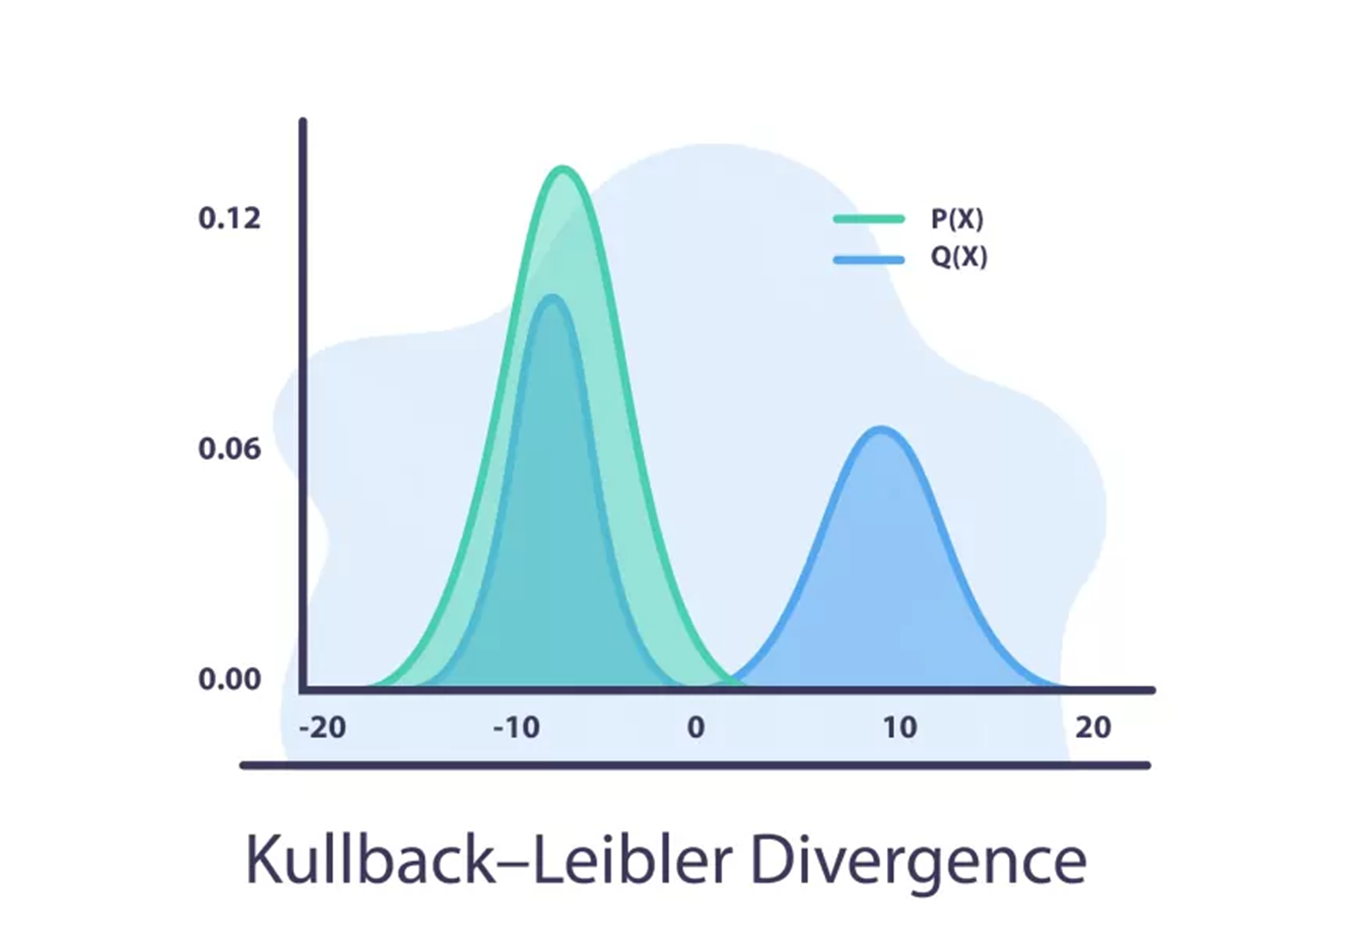
\includegraphics[width=1\linewidth]{imagens/kl_divergence.png}
        \centering\caption*{ $$D_{\text{KL}}(p(x) || q(x)) = \int p(x) \ln \left( \frac{p(x)}{q(x)} \right) dx$$}
    \end{minipage}%
    \begin{minipage}{.5\textwidth}
        \centering
        \includegraphics[width=1\linewidth]{imagens/action_based.png}
        \caption*{Markov Blanket States}
    \end{minipage}
\end{figure}
\end{frame}

\subsection{Hebbian Learning}
\begin{frame}{2.2 Hebbian Learning \cite{albanese2024hebbian}}

\begin{itemize}
    \item Hebbian learning is a learning mechanism inspired by the brain's plasticity, where the connection between neurons is strengthened if they are activated simultaneously.

    \item Main idea: “\textbf{\textit{Neurons that fire together, wire together}}”.
\\→ Neurons that fire out of sync lose their link. 
\end{itemize}
The basic premise of Hebbian Learning is encapsulated in the formula:

$$\Delta w = \eta xy$$

where:

\begin{itemize}
 \item $\Delta w$ is the change in the weight of the synapse,
 \item $\eta$ is the learning rate, a small positive scalar that determines the step size of the weight update,
 \item $x$ is the presynaptic neuron's activity level, and
 \item $y$ is the postsynaptic neuron's activity level.
\end{itemize}

\end{frame}


\section{Classic \& Modern learning mechanisms}
\subsection{Classic Hopfield Network}
\begin{frame}{3.1. Classic Hopfield Network \cite{Hopfield:2007}}
    \begin{itemize}
        \item Stored patterns: $\{x_i\}^N_{i=1}$, where:
        \begin{itemize}
            \item $N$: number of stored patterns.
            \item $x_i$ must be a polar pattern with d elements.
        \end{itemize}

        \item Weight matrix: $$W = \sum_i^N x_i x_i^T$$

        \item Main goal: Retrieving the original pattern from a noisified one.

    \end{itemize}
\end{frame}

\begin{frame}{3.1.1 Synchronous}
\textbf{Update rule}: Update pattern \( S \) according to the following formula:
\[
S^{t+1} = \text{sgn}(W S^t - b),
\]
where:
\begin{itemize}
    \item \(\text{sgn}(\cdot)\): sign function.
    \item \( b \): bias vector (typically \( \vec{0} \)).
    \item \( S^t \): state pattern at the \( t \)-th update.
\end{itemize}
Convergence occurs when \( S^{t+1} = S^t \).

\end{frame}

\begin{frame}{3.1.2 Asynchronous}
\textbf{Energy function}:
\[
E(S) = -\frac{1}{2} S^T W S + S^T b
\]
\textbf{Update rule}: Update the components \( s_i \) of the vector \( S \) according to the formula:
\[
s_i = \text{sgn}(W s_i - b),
\]
where:
\begin{itemize}
    \item \( s_i \): the \( i \)-th component of the pattern \( S \).
\end{itemize}
Convergence is achieved when \( S \) is a local minima of the function \( E(S) \).

\end{frame}

\begin{frame}{3.1. Classic Hopfield Network \cite{Hopfield:2007}}
    \( d \) is the dimension of the input.
    
\textbf{Limitations}

\begin{itemize}
    \item Small memory capacity: $C \approx 0.14d$.
    \item Not reliable enough in retrieving original patterns.
    \item Only support polar (binary) patterns.
\end{itemize}
\end{frame}

\subsection{Modern Hopfield Network}
\begin{frame}{3.2. Modern Hopfield Network}

\textbf{Krotov and Hopfield introduced the energy function}:
\[
E = -\sum_{x=1}^N F(x_i^T S),
\]
where $F(z) = z^\alpha$ is a polynomial interaction function and \( N \) is the number of stored patterns.

\textbf{New update rule}:
\[
S^{\text{new}}[l] = \text{sgn} \left[ -E(S^{(l+)}) + E(S^{(l-)}) \right],
\]
\end{frame}

\begin{frame}{3.2. Modern Hopfield Network}
\begin{figure}
    \centering
    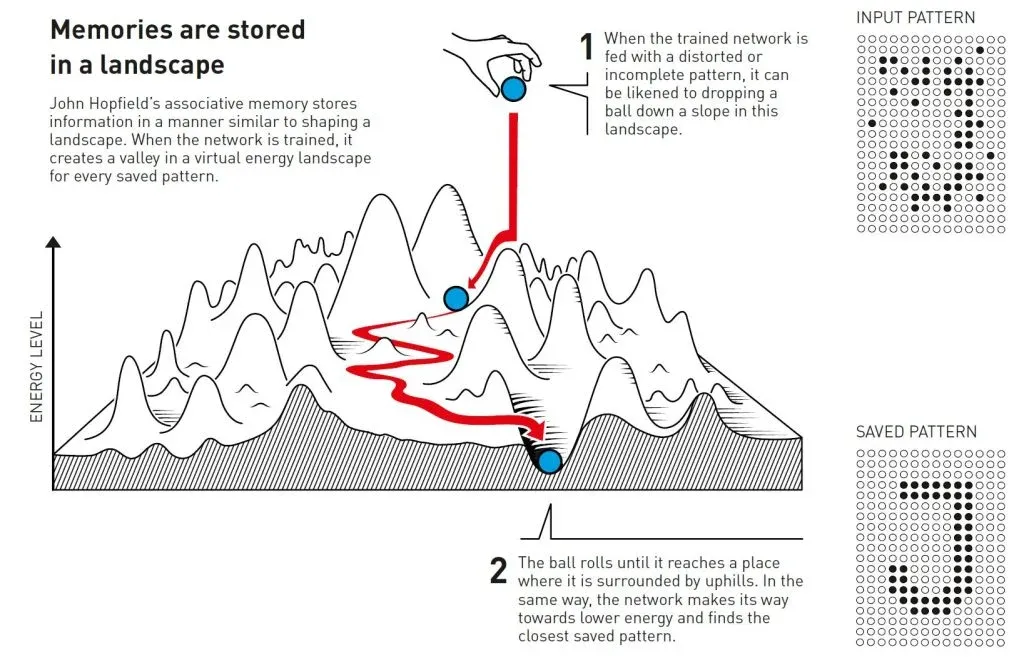
\includegraphics[width=0.65\linewidth]{imagens/concept_2.png}
    \caption{Pattern approaching local minima}
    \label{fig:motivation_2}
\end{figure}
\end{frame}

\begin{frame}{3.2. Modern Hopfield Network}
\textbf{Pros: }
\begin{itemize}
    \item Memory capacity is much higher: $C = \dfrac{1}{2(2\alpha - 3)!!}\dfrac{d^{\alpha - 1}}{log(d)}$.
    \item Achieves convergence after one update.
\end{itemize}
\textbf{Cons:}
\begin{itemize}
    \item Might converge to incorrect local minima. 
\end{itemize}

\end{frame}

\section{Application}
\begin{frame}{4. Application}
    \begin{itemize}
        \item Associative Memory for Image Reconstruction (Simpson Dataset).
    \end{itemize}

    \begin{figure}
        \centering
        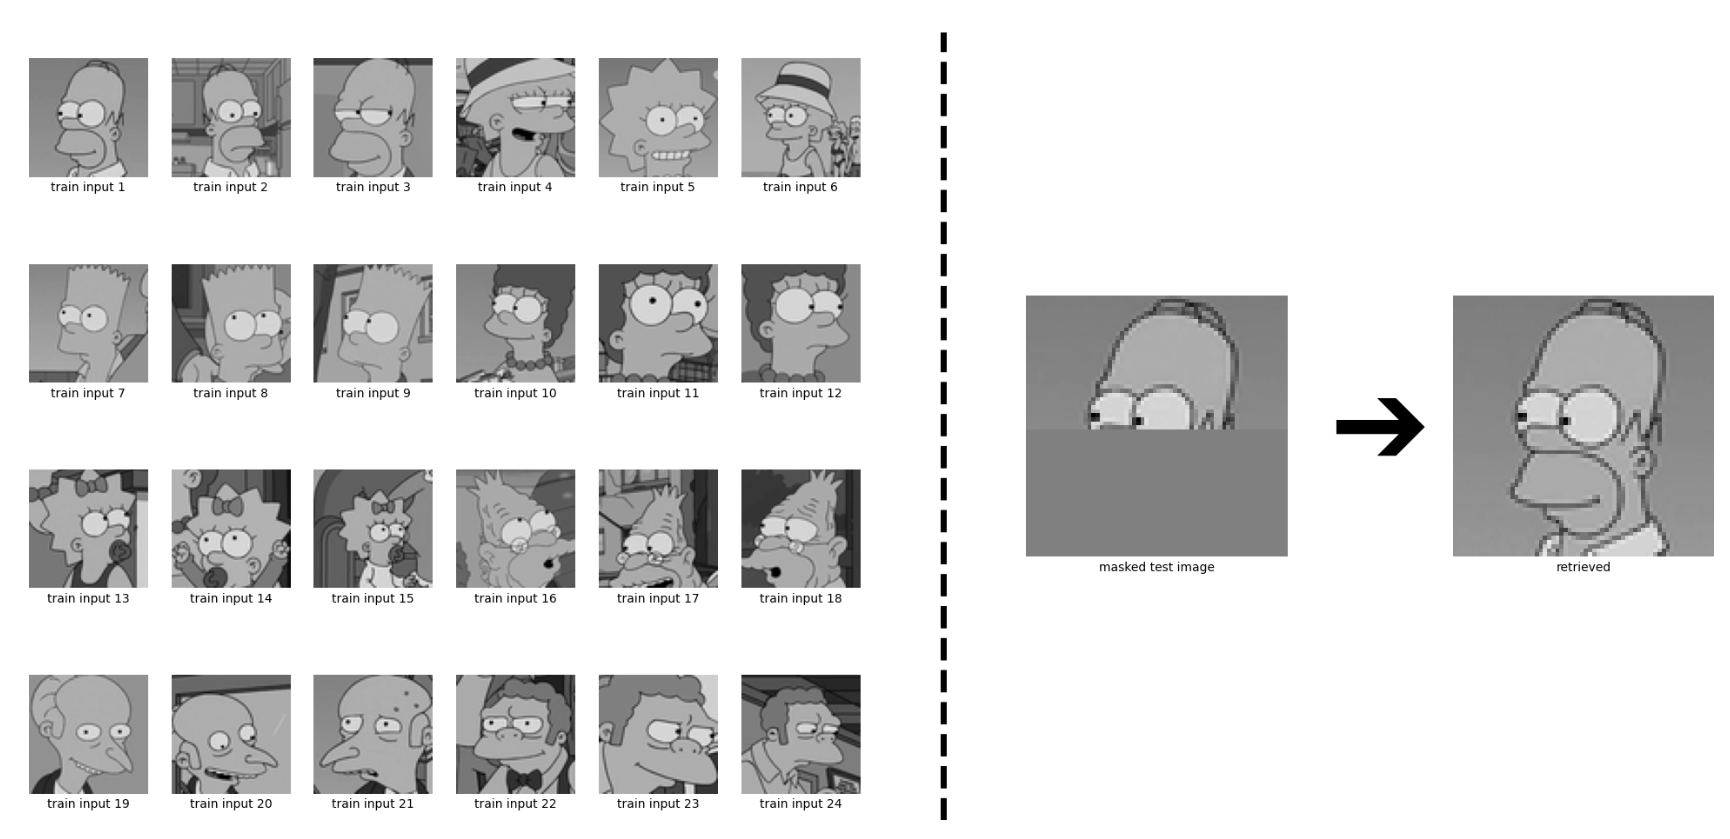
\includegraphics[width=0.7\linewidth]{imagens/simpson_2.png}
        \caption{Image Reconstruction}
        \label{fig:simpson}
    \end{figure}
\end{frame}
\begin{frame}{4. Application}
    \begin{itemize}
        \item Hopfield Attention \cite{vaswani2017attention}.
    \end{itemize}
    \begin{figure}[H]
        \centering
        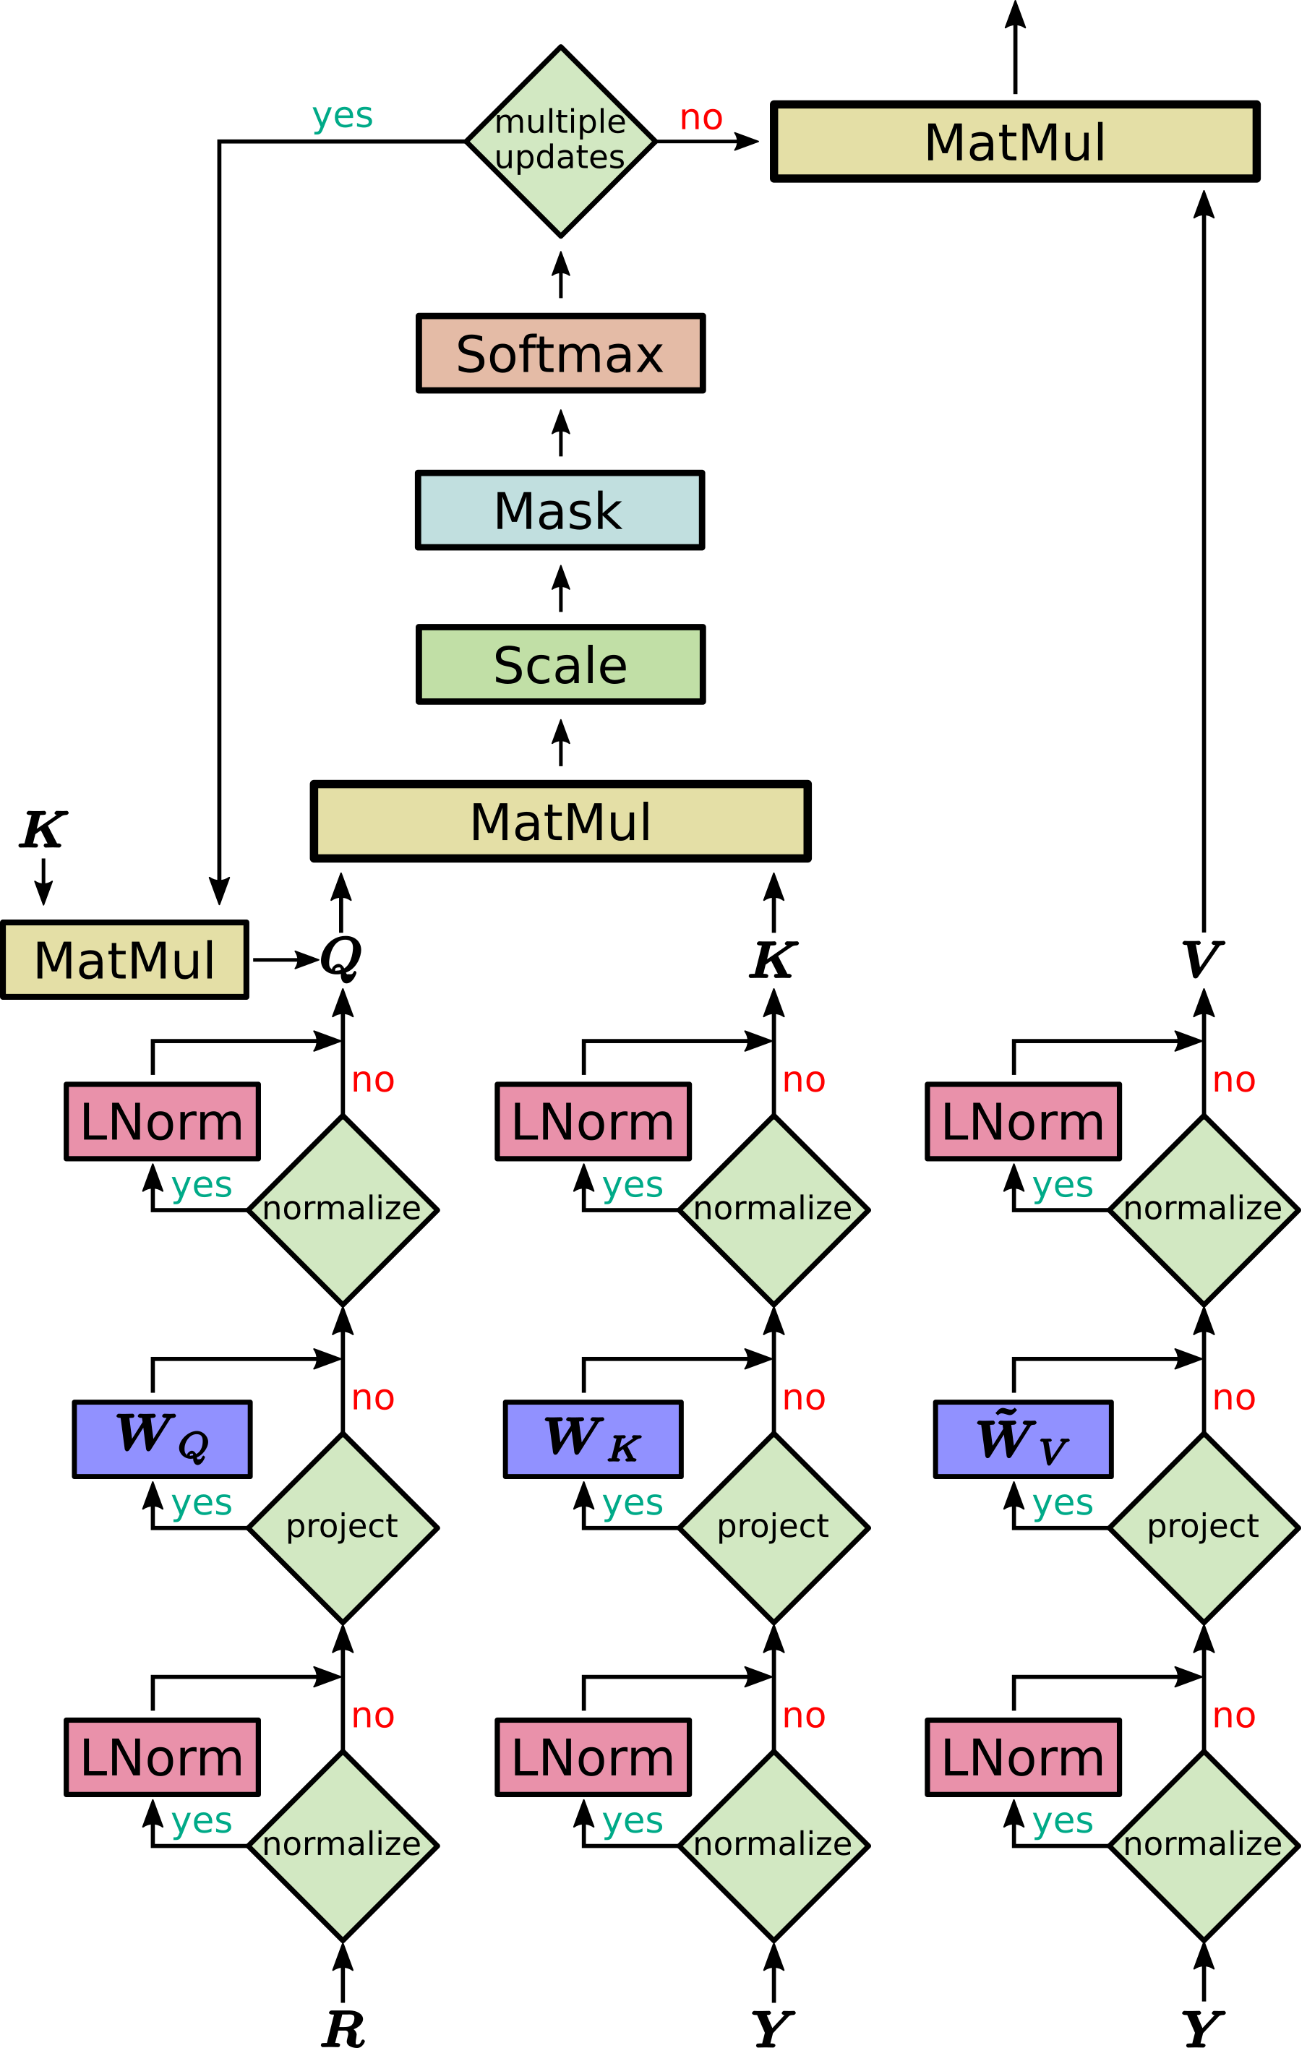
\includegraphics[width=0.25\linewidth]{imagens/hopfield_attention_2.png}
        \caption{Hopfield Attention}
    \end{figure}
\end{frame}

\begin{frame}{4. Application}
    \begin{itemize}
        \item NP-hard solver (N-queens problem) \cite{nqueens}.
    \end{itemize}
    \begin{figure}
        \centering
        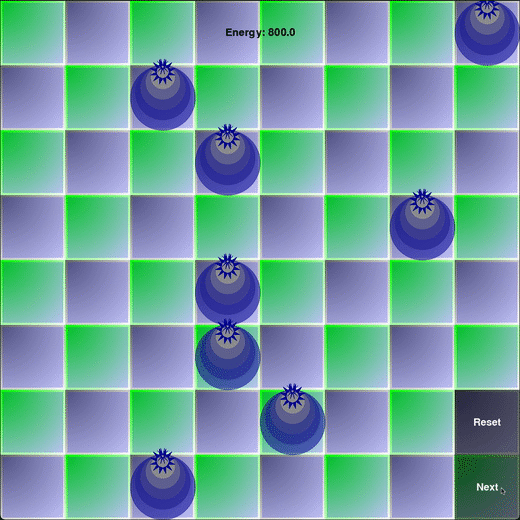
\includegraphics[width=0.4\linewidth]{imagens/nqueens.png}
        \caption{N-queens problem}
        \label{fig:queen}
    \end{figure}
    % \begin{figure}[H]
    %     \centering
    %     \begin{minipage}{.5\textwidth}
    %         \centering
    %         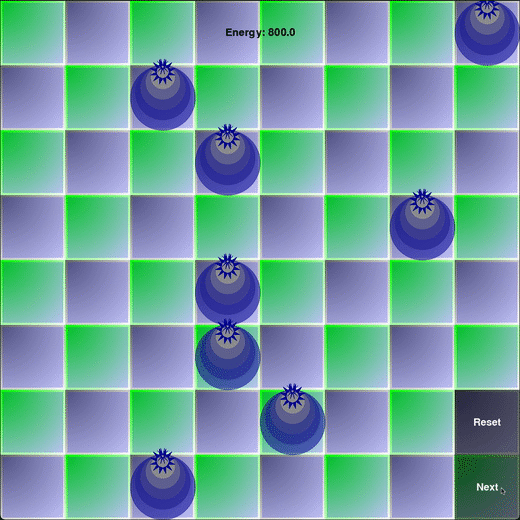
\includegraphics[height=1.2in]{imagens/nqueens.png}
    %         \caption*{N-queens}
    %     \end{minipage}%
    %     \begin{minipage}{.5\textwidth}
    %         \centering
    %         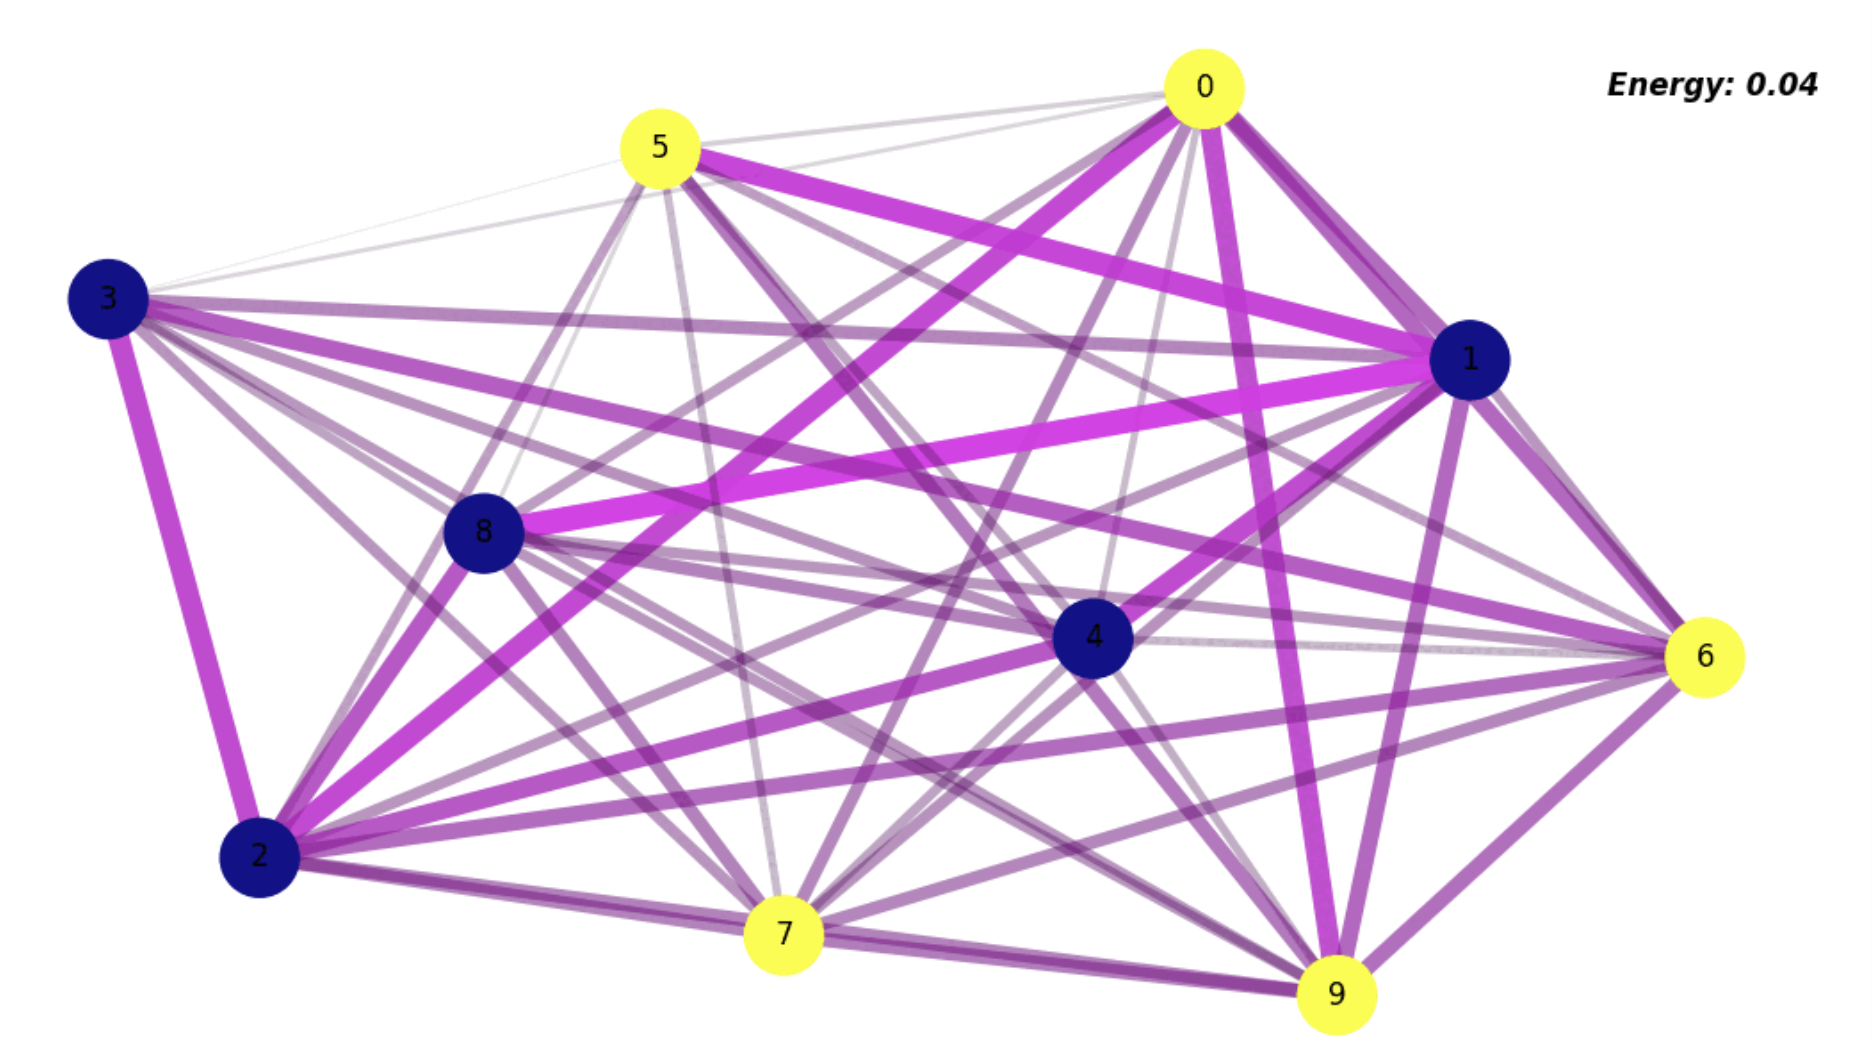
\includegraphics[height=1.2in]{imagens/tsp.png}
    %         \caption*{TSP}
    %     \end{minipage}
    %     \caption{NP-hard problems}
    % \end{figure}
\end{frame}

\subsection{N-queens problem solver}
\begin{frame}{4.3 N-queens problem solver}
The N-queens problem is a classic combinatorial problem where the goal is to place n chess queens on an n x n chessboard such that no two queens threaten each other.
% This section provides a concise overview of the application of a Hopfield network to solving the N-Queens problem.
\begin{figure}[H]
    \centering
    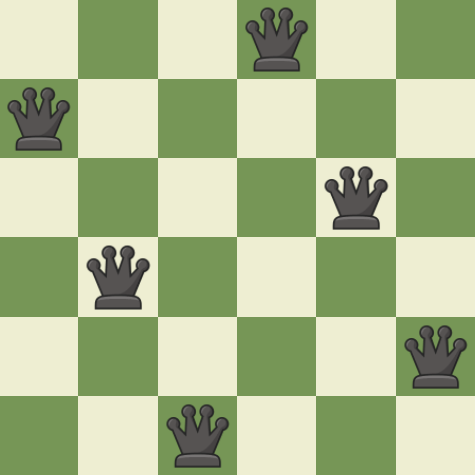
\includegraphics[width=0.4\linewidth]{imagens/nqueen.png}
    \caption{N-queens}
    \label{fig:nqueens2}
\end{figure}
\end{frame}

\begin{frame}{4.3 N-queens problem solver}
The Hopfield network model used is the classical binary Hopfield model, modified to be suitable for solving the N-Queens problem. \\
Compared to the original model, this model has the following main differences:
\begin{itemize}
    \item Completely binary.
    \item Random initialization.
    \item Modified energy function and input potential computation.
\end{itemize}
\textbf{Goal}: Find a state configuration that minimizes the energy function, or ideally, makes the energy function equal to zero.
\end{frame}

\begin{frame}{4.3 N-queens problem solver}
\framesubtitle{Energy function}
The \textbf{energy function} $E$ is defined as follows:
\begin{align*} 
E &= \frac{1}{2} \sum_{i=1}^n \sum_{j=1}^n \left[ A \cdot R_{ij} + B \cdot D_{ij}\right] + \frac{1}{2}C\left(\sum_{i=1}^n \sum_{j=1}^n v_{ij} - (n + \sigma)\right)^2
\end{align*}
Where:
\begin{itemize}
    \item $R_{ij}=\left(\sum_{k\ne j}v_{ik} + \sum_{k\ne i}v_{kj}\right)v_{ij}$
    (penalizes when there is more than one Queen in the same row or column)
    \item $D_{ij} = \left(\sum_{(k, l) \in \text{diagonal of }(i, j)}v_{kl}\right)v_{ij}$
    (penalizes if there is another Queen on the same diagonal)
    \item $\sum v_{ij}$: Total number of Queens on the board
\end{itemize}
\end{frame}

\begin{frame}{4.3 N-queens problem solver}
\framesubtitle{Output potential function}
Binary threshold function to compute the \textbf{output potential} of the neuron:
\[
v(u) = \begin{cases} 0 & \text{if } u < 0 \\ 1 & \text{if } u \ge 0 \end{cases}
\]
\end{frame}

\begin{frame}{4.3 N-queens problem solver}
\framesubtitle{Input potential function}
Given the \textbf{input potential} of the neuron $(i, j)$ at time $t$, the formula for the input potential $U_{ij}(t)$ is:
\begin{equation}
U_{ij}(t) = -A \cdot H_{ij}(t) - R_{ij}(t) - S_{ij}(t) - C \cdot \left( \sum V_{kl}(t) - (n + \sigma) \right)
\end{equation}

\begin{itemize}
    \item \( H_{ij}(t) = \sum_{k \neq j} V_{ik}(t) + \sum_{k \neq i} v_{kj}(t) \): Sum of states over rows and columns
    \item \( R_{ij}(t) \): Off-diagonal interaction force (when \( i - j = \text{const} \))
    \item \( S_{ij}(t) \): Sum of on-diagonal interaction forces (when \( i + j = \text{const} \))
    \item \( \sum v_{kl}(t) \): Total number of queens on the board at time \( t \)
\end{itemize}
\end{frame}

\begin{frame}{4.3 N-queens problem solver}
\framesubtitle{Experimentation}
Due to limitations in time and computational resources, we conducted experiments with 4, 8, and 16 queens. For each configuration, we performed 100 runs and calculated the convergence rate of that configuration.\\
We will employ three network initialization strategies:
\begin{itemize}
    \item \textbf{Strategy 1}: All neurons set to 0.
    \item \textbf{Strategy 2}: Neurons randomly set to 0 or 1.
    \item \textbf{Strategy 3}: All neurons set to 1.
\end{itemize}
\end{frame}

\begin{frame}{4.3 N-queens problem solver}
\framesubtitle{Experimentation}
Due to limitations in time and computational resources, we conducted experiments with 4, 8, and 16 queens. For each configuration, we performed 100 runs and calculated the convergence rate of that configuration.\\
We will employ three network initialization strategies:
\begin{itemize}
    \item \textbf{Strategy 1}: All neurons set to 0.
    \item \textbf{Strategy 2}: Neurons randomly set to 0 or 1.
    \item \textbf{Strategy 3}: All neurons set to 1.
\end{itemize}

\end{frame}

\begin{frame}{4.3 N-queens problem solver}
\framesubtitle{Experimentation}
\begin{table}
    \centering
    \begin{tabular}{|c|c|c|c|}
        \hline
        & Strategy 1 & Strategy 2 & Strategy 3 \\
        \hline
        \( n = 4 \) & 100\% & 100\% & 100\% \\
        \( n = 8 \) & 100\% & 99\% & 100\% \\
        \( n = 16 \) & 100\% & 100\% & 100\% \\
        \hline
    \end{tabular}
    \caption{A = B = C = 100 and \(\sigma = 0\) (asynchronous mode)}
\end{table}

\begin{table}
    \centering
    \begin{tabular}{|c|c|c|c|}
        \hline
        & Strategy 1 & Strategy 2 & Strategy 3 \\
        \hline
        \( n = 4 \) & 100\% & 100\% & 100\% \\
        \( n = 8 \) & 98\% & 100\% & 97\% \\
        \( n = 16 \) & 100\% & 100\% & 99\% \\
        \hline
    \end{tabular}
    \caption{A = B = 100, C = 40 and \(\sigma = 2\) (synchronous mode)}
\end{table}

\end{frame}

\begin{frame}{4.3 N-queens problem solver}
\framesubtitle{Experimentation}
\begin{table}
    \centering
    \begin{tabular}{|c|c|c|c|}
        \hline
        & Strategy 1 & Strategy 2 & Strategy 3 \\
        \hline
        \( n = 4 \) & 100\% & 100\% & 100\% \\
        \( n = 8 \) & 100\% & 100\% & 100\% \\
        \( n = 16 \) & 100\% & 100\% & 100\% \\
        \hline
    \end{tabular}
    \caption{A = 100, B = 50, C = 100 and \(\sigma = 0\) (asynchronous mode)}
\end{table}

\begin{table}
    \centering
    \begin{tabular}{|c|c|c|c|}
        \hline
        & Strategy 1 & Strategy 2 & Strategy 3 \\
        \hline
        \( n = 4 \) & 18\% & 17\% & 27\% \\
        \( n = 8 \) & 4\% & 5\% & 7\% \\
        \( n = 16 \) & 3\% & 1\% & 2\% \\
        \hline
    \end{tabular}
    \caption{A = B = 100, C = 40 and \(\sigma = 0\) (synchronous mode)}
\end{table}
\end{frame}

\begin{frame}{4.3 N-queens problem solver}
\framesubtitle{Time complexity}
Calculating the complexity for this problem is very challenging. In the original paper, the author estimated the complexity experimentally with the following results:
\begin{itemize}
    \item Asynchronous mode: \( O(n^{4.47}) \)
    \item Synchronous mode: \( O(n^{4.67}) \)
\end{itemize}
\end{frame}

\begin{frame}{4.3 N-queens problem solver}
\framesubtitle{Advantages and disadvantages}
\begin{itemize}
    \item \textbf{Advantages:}
    \begin{itemize}
        \item High convergence rate
        \item Effective for NP-Hard problems
        \item Stability
    \end{itemize}
    \item \textbf{Disadvantages:}
    \begin{itemize}
        \item Hyperparameter tuning required
        \item Complex energy function
    \end{itemize}
\end{itemize}
\end{frame}
\subsection{Wordle solver}
\begin{frame}{4.4 Wordle}
    \begin{itemize}
        \item Wordle.
    \end{itemize}
    \begin{figure}[H]
        \centering
        \begin{minipage}{.5\textwidth}
            \centering
            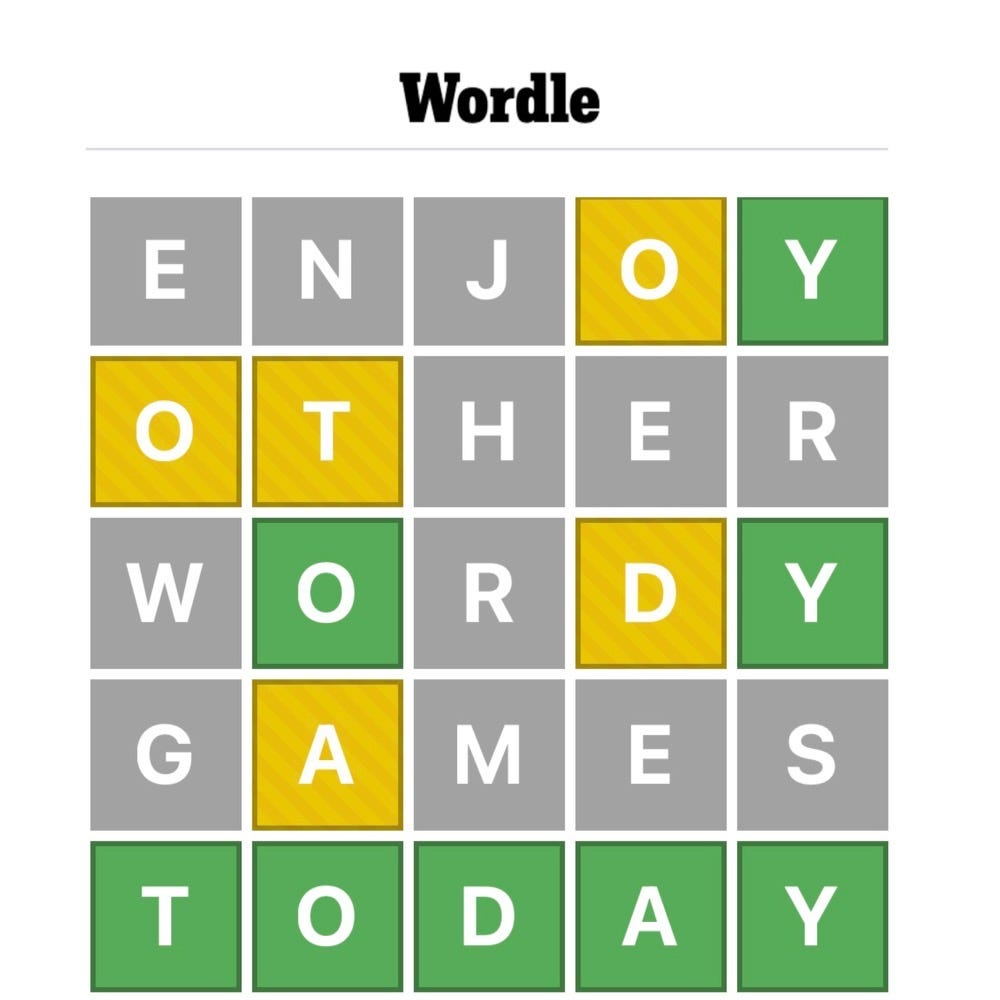
\includegraphics[height=1.7in]{imagens/wordle.jpg}
        \end{minipage}%
        \begin{minipage}{.5\textwidth}
            \centering
            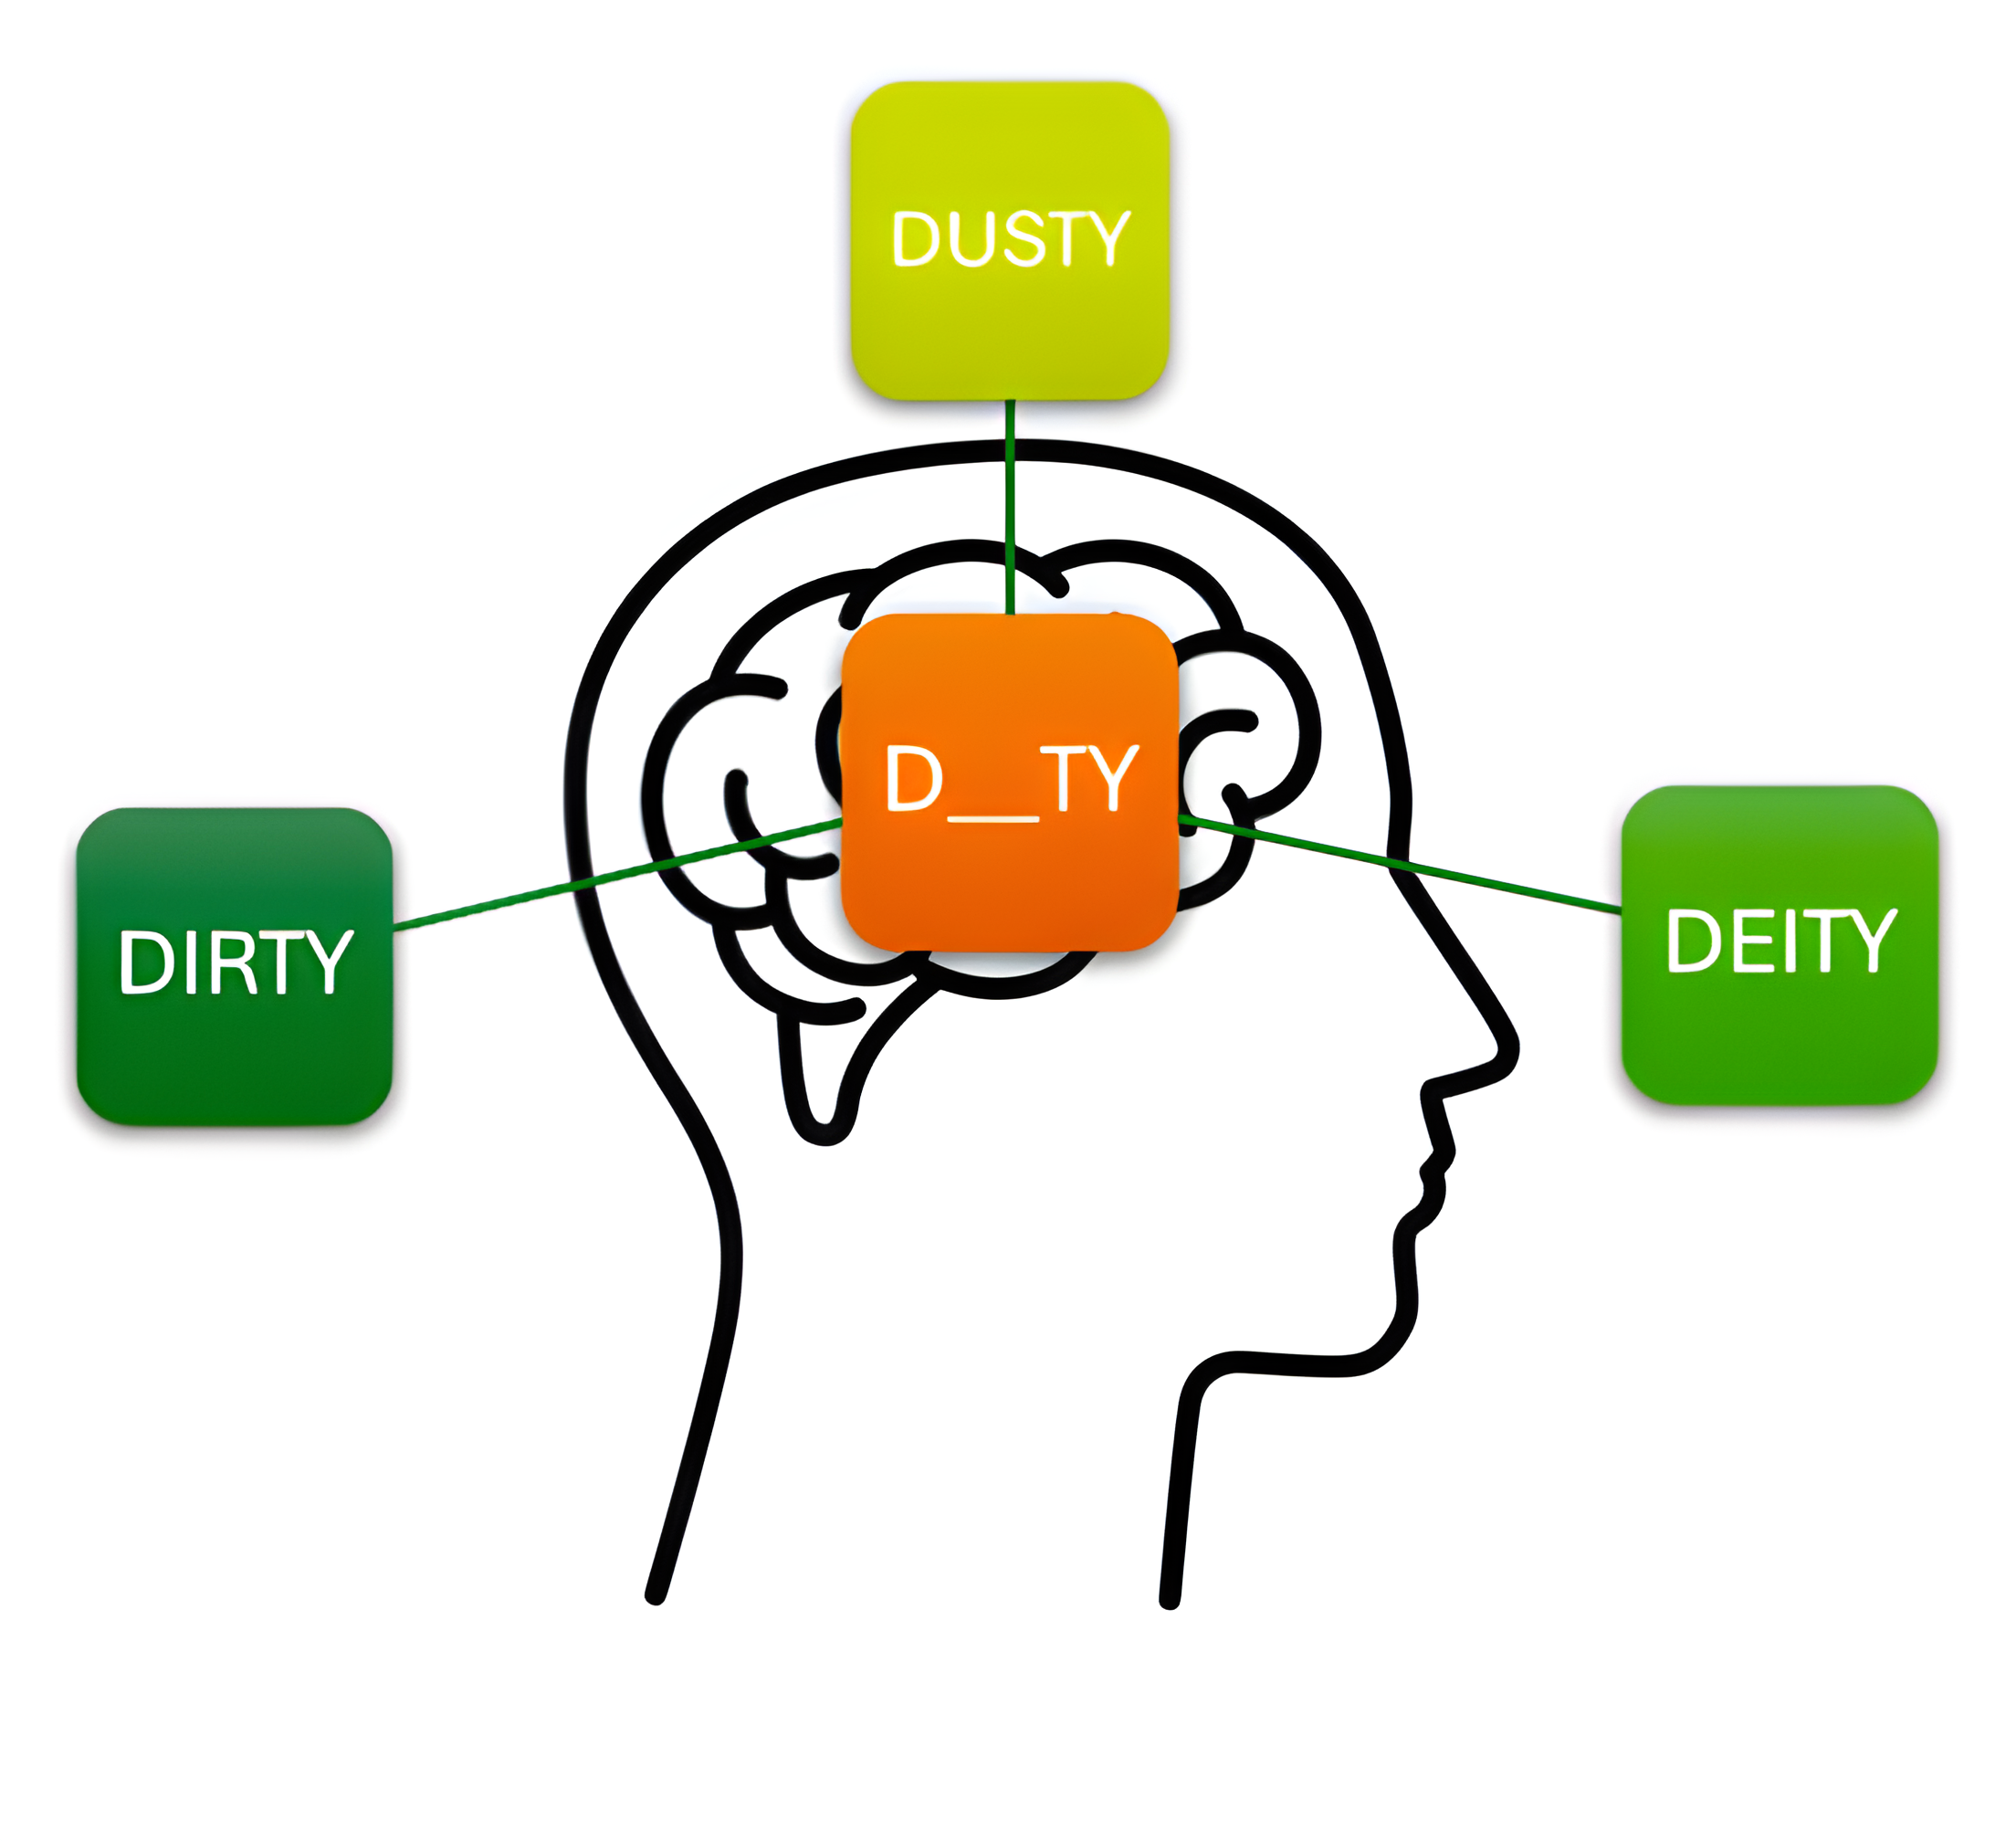
\includegraphics[height=1.7in]{imagens/thinking.png}
        \end{minipage}
        \caption{Wordle}
    \end{figure}
\end{frame}

\begin{frame}{4.4 Wordle}
\framesubtitle{Methodology}
    \begin{itemize}
        \item Wordle.
    \end{itemize}
    \begin{figure}[H]
        \centering
        \begin{minipage}{.6\textwidth}
            \centering
            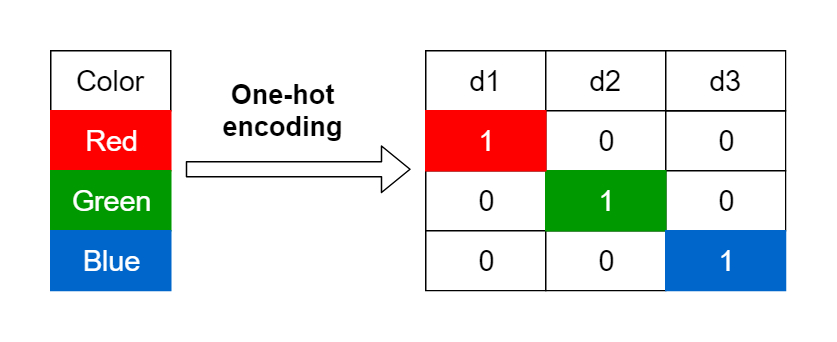
\includegraphics[height=1.1in]{imagens/onehot.jpg}
        \end{minipage}%
        \begin{minipage}{.4\textwidth}
            \centering
            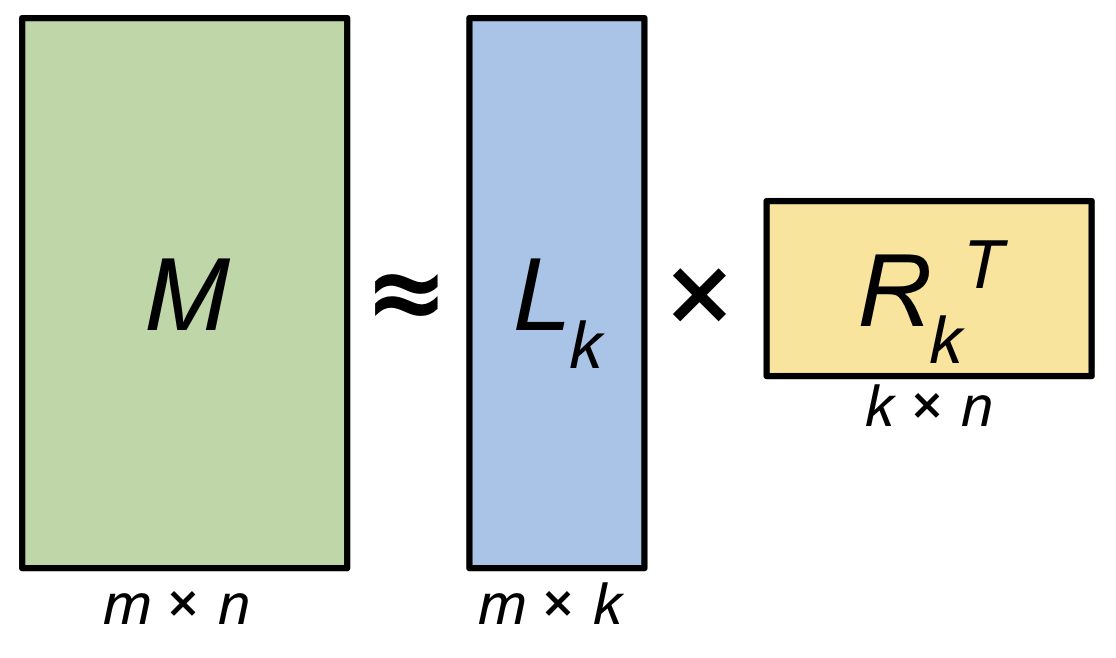
\includegraphics[height=0.9in]{imagens/low-rank-approximation.png}
        \end{minipage}
        \caption{Method}
    \end{figure}
\end{frame}

\begin{frame}{4.4 Wordle}
\framesubtitle{Result \& Ideas}
\textbf{Result}: Failed
\begin{itemize}
    \item Sub-optimal energy minima: Cause the network to converge into nonsensible words.
    \item Suppress mechanism for newly recalled words: Delete permanently from memories. $\implies$ Unstable, cause havoc and chao.
\end{itemize}

\textbf{Ideas}: 
\begin{itemize}
    \item Inhibitory field in Hopfield.
    \item Dense distributed representation.
    HElp me
\end{itemize}
\end{frame}

%----------------------------------------------

% \section{Plans}
% \begin{frame}{5. Plans}
%     \begin{itemize}
%         \item Deep reading, summarize key ideas for the report (all members).
%         \item Write core theory sections, start coding implementation.
%         \begin{itemize}
%             \item Implementing base models (An).
%             \item \href{https://github.com/AnhKhoa585/hopfield-npHard}{\textbf{NP-hard solver}} (Khoa).
%             \item Associative Memory for Image Reconstruction (An).
%             \item \textbf{\href{https://github.com/sabertoaster/HopfieldWordle}{Hopfield Wordle}} (Huy).

%         \end{itemize}
%         \item Run experiments, collect results (all members).
%         \item Complete the report (Hong).
%         \item Prepare presentation slides (all members).
%         \item Record and edit 10–15 mins presentation video (all members).
%         \item Review formatting, references, and finalize all files (all members).
%     \end{itemize}
% \end{frame}
\section{References}
\begin{frame}[allowframebreaks]{6. References}
    \bibliography{./references}
\end{frame}


% \section{Conteúdo}

% \begin{frame}{Definições, Teoremas, Corolários e Exemplos}
%     \begin{block}{Definição 2.1.1}
%     Aqui temos uma nova definição.
%     \end{block}
    
%     \begin{block}{Teorema 2.1.2}
%     Aqui temos um novo teorema.
%     \end{block}
    
%     \begin{block}{Exemplo 2.1.3}
%     Aqui temos um novo exemplo.
%     \end{block}
    
%     \begin{block}{Corolário 2.1.4}
%     Aqui temos um novo corolário.
%     \end{block}
% \end{frame}

% \begin{frame}{Citações das Referências}
%     Livro de Análise Real~\cite{lima2004analise}
% \end{frame}

% \begin{frame}{Listas}
%     Exemplo de lista com símbolos:

%     \begin{itemize}
%         \item Primeiro elemento
%         \item Segundo elemento
%     \end{itemize}
    
%     \bigskip
    
%     Exemplo de lista com itens enumerados:
    
%     \begin{enumerate}
%         \item Primeiro elemento
%         \item Segundo elemento
%     \end{enumerate}
% \end{frame}

% \begin{frame}{Tabelas}
%     A Tabela mostra um modelo de tabela.

%     \begin{table}[htb]
%         \caption{Exemplo de tabela}
%         \label{tab:modelo_tabela}
%         \centering
%         \begin{tabular}{c|c|c|c}
% 	        \hline
% 	        \textbf{Pessoa} & \textbf{Idade} & \textbf{Peso} & \textbf{Altura} \\ \hline
% 	        Marcos & 26    & 68   & 178    \\ \hline
% 	        Ivone  & 22    & 57   & 162    \\ \hline
% 	        Sueli  & 40    & 65   & 153    \\ \hline
%         \end{tabular}
        
%         \medskip
        
%         Fonte: Produção do próprio autor.
%     \end{table}
% \end{frame}

% \begin{frame}{Imagens}
%     A Figura mostra a logomarca promocional da Universidade Federal do Espírito Santo (UFES).
    
%     \begin{figure}[htb]
%         \caption{Logomarca Promocional UFES}
%         \label{fig:logo_UFES}
%         \centering
%         
\includegraphics[width=0.5\textwidth]{imagens/logomarca_UFES}
        
%         \medskip
        
%         Fonte: Produção do próprio autor.
%     \end{figure}
% \end{frame}

% \begin{frame}{Conclusão}
%     Texto referente à conclusão.
% \end{frame}

% \begin{frame}{Trabalhos futuros}
%     \begin{itemize}
%         \item Estudar $\ldots$
        
%         \medskip
        
%         \item Explorar $\ldots$
        
%         \medskip
        
%         \item Analisar $\ldots$
%     \end{itemize}
% \end{frame}

% \section{Referências}
% \begin{frame}[allowframebreaks]{Referências}
%     \bibliography{referencias}
% \end{frame}

% \begin{frame}

% \begin{center}
%     Obrigado!
    
%     \email
% \end{center}

% \begin{figure}[htb]
%     \centering
%     
\includegraphics[width=0.5\textwidth]{imagens/logomarca_UFES}
% \end{figure}

% \end{frame}

\end{document}